% !TeX root = ../../main.tex
\documentclass[../../main.tex]{subfiles}
\begin{document}

\chapter{Variables in \LaTeX}

Variables are destroyed after endgroup. (begingroup - endgroup)

%----------------------------------------------
\section{Simple Text Variables in tables}

\begingroup
    % Define "variables" (macros) for table cells using \def or \newcommand
    \def\cellA{\textbf{Apple}}
    \def\cellB{\textcolor{red}{Fruit}}
    \def\cellC{\textbf{Carrot}}
    \def\cellD{\textcolor{orange}{Vegetable}}
    
    % Now use these variables inside a table
    \begin{center}
        \begin{tabular}{|c|c|}
        \hline
        \cellA & \cellB \\ \hline
        \cellC & \cellD \\ \hline
        \end{tabular}
    \end{center}
    \medskip
    % After \endgroup, macros \cellA, \cellB, etc. are no longer defined.
\endgroup}

\lstinputlisting[
    language=TeXish,
    linerange={1-19}
]{\subfix{example_codes/variable_table_example.tex}}

\clearpage

\section{Simple Text Variables}

\begingroup
\centering

\newcommand{\varText}{\textbf{Text Variable}.}
\medskip
\varText

\endgroup}

\lstinputlisting[
    language=TeXish,
    linerange={4-4}
]{\subfix{example_codes/variable_text.tex}}

\section{Simple Maths Variables}

\begingroup
\centering

\def\varMath{$E = mc^2$}   \varMath

\endgroup}

\lstinputlisting[
    language=TeXish,
    linerange={4-4}
]{\subfix{example_codes/variable_maths.tex}}

\section{Simple tikz image Variables}

\begingroup
    \newsavebox{\figBox}
    \begin{lrbox}{\figBox}
        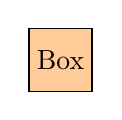
\begin{tikzpicture}[scale=0.8]
            \draw[fill=orange!40] (2.5,0) rectangle (3.5,1);
            \node at (3,0.5) {Box};
        \end{tikzpicture}
    \end{lrbox}

    \begin{figure}[h]
        \centering
        \usebox{\figBox}
        \caption{Stored Figure}
    \end{figure}
\bigskip
\endgroup}

\lstinputlisting[
    language=TeXish,
    linerange={1-16}
]{\subfix{example_codes/variable_figure.tex}}

\clearpage

\section{Simple Table Variables}

\begingroup
	\newsavebox{\tableBox}
	\begin{lrbox}{\tableBox}
		\begin{tabular}{|c|c|} \hline
			\textbf{Fruit} & \textbf{Color} \\ \hline
			Apple & Red \\ \hline
		\end{tabular}
	\end{lrbox}

	\begin{center}
		\usebox{\tableBox}\\[3pt]
		\textbf{Stored Figure}
	\end{center}
\endgroup}

\lstinputlisting[
    language=TeXish,
    linerange={1-16}
]{\subfix{example_codes/variable_table.tex}}

\section{Dynamic content variable using newtoks}

\begingroup
    \newtoks\varTokens
    \varTokens={This is \textit{stored} in a token register.}
    \the\varTokens
\endgroup}

\lstinputlisting[
    language=TeXish,
    linerange={1-5}
]{\subfix{example_codes/variable_newtoks.tex}}


\section{Temporary macros (auto-destroyed after scope)}

\begingroup
    \def\tempA{Scoped \textbf{variable A}}
    \medskip
    \noindent \tempA 
\endgroup}

\lstinputlisting[
    language=TeXish,
    linerange={1-5}
]{\subfix{example_codes/variable_macros.tex}}

\end{document}
